\section{Problem 3: Derandomizing Signatures}\label{sec:problem3}

Let $\mathcal{S} = (G, S, V)$ be a secure signature scheme defined over $(\mathcal{M}, \Sigma)$, where the signing algorithm $S$ is probabilistic.
In particular, algorithm $S$ uses randomness chosen from a space $\mathcal{R}$.
We let $S(sk,m;r)$ denote the execution of algorithm $S$ with randomness $r$.
Let $F$ be a secure PRF defined over $(\mathcal{K}, \mathcal{M}, \mathcal{R})$.
Show that the following signature scheme $\mathcal{S'} = (G', S', V)$ is secure:
\begin{equation*}
    \begin{split}
        G'() &\coloneqq \{ (pk, sk) \overset{\mathcal{R}}{\longleftarrow} G(), 
            \hspace{3pt} k \overset{\mathcal{R}}{\longleftarrow} \mathcal{K}, 
            \hspace{3pt} sk' \coloneqq (sk, k), 
            \hspace{3pt} \text{output } (pk, sk') \}; \\
        S'(sk', m) &\coloneqq \{ r \longleftarrow F(k, m),
            \hspace{3pt} \sigma \longleftarrow S(sk, m; r),
            \hspace{3pt} \text{output } \sigma \}.
    \end{split}
\end{equation*}
Now the signing algorithm for $S'$ is deterministic.

\begin{center}
    \rule{5cm}{0.4pt}
\end{center}

\textbf{\textit{Proof:}}
Let us denote, for the sake of simplicity, as $S_{R}$ the \textit{randomized} signature scheme, and as $S_{DR}$ the \textit{derandomized}.
Our hypothesis is that $S_R$ is secure against a chosen message attack, as defined in the Attack Game $13.1$, and that $F$ is a secure $PRF$, as defined in Attack Game $4.2$.

We will assume that $S_{DR}$ is \emph{not} secure, and find that this will contradict one of our hypothesis.
In particular, assuming the existence of an attacker $\mathcal{A}_{DR}$ that wins game $13.1$, we will generate a forgery to win the same game for $S_R$.
The scheme is depicted in Figure \ref{fig:attack-game}

\begin{figure}[h!]
    \centering
    \begin{tikzpicture}
        % Define Variables
        \def\lR{0.75}
        \def\rR{5.35}
        \def\lDR{10.75}
        \def\rDR{15.35}
        \def\bottom{-9}

        % Overall Scheme
        \draw[thick] (0,0) -- (6,0) node[midway, anchor=south] {Randomized Game};
        \node[anchor = north west] at (0,0) (c-r) {\scriptsize Challenger};
        \draw[dotted] (\lR, -0.5) -- (\lR,\bottom);
        \node[anchor = north east, text=red] at (6,0) {\scriptsize Attacker};
        \draw[dotted] (\rR, -0.5) -- (\rR, \bottom);
        \draw[thick, dashed] (6,0) -- (6, \bottom);
        \draw[thick] (10,0) -- (16,0) node[midway, anchor=south] {De-Randomized Game};
        \node[anchor = north west, text=red] at (10,0) {\scriptsize Challenger};
        \node[anchor = north east, text=blue] at (16,0) {\scriptsize Attacker};
        \draw[thick, dashed] (10,0) -- (10, \bottom);
        \draw[dotted] (\lDR, -0.5) -- (\lDR, \bottom);
        \draw[dotted] (\rDR, -0.5) -- (\rDR, \bottom);

        % Start Games
        \draw[->] (\rR, -1) -- (\lR, -1) node[midway, anchor=south] {\scriptsize Start Game};
        \draw[->] (\lR, -1.75) -- (\rR, -1.75) node[midway, anchor=south] {};
        \node[anchor=west] at (\lR, -1.5) {$(pk, sk) \overset{\mathcal{R}}{\longleftarrow} G()$};
        \node[anchor=east] at (\rR, -1.5) {$pk$};
        \draw[->,color=red] (\rR, -2) -- (\lDR, -2) node[anchor=north east, text=red] {$pk$};
        \draw[->] (\lDR, -2.25) -- (\rDR, -2.25) node[anchor=south east, text=blue] {$pk$};

        % First Signing Query
        \draw[->] (\rDR, -2.75) -- (\lDR, -2.75) node[midway, anchor=south] {\scriptsize $Sign(m_1)$};
        \node[anchor=north east, text=blue] at (\rDR, -2.75) {$m_1$};
        \draw[->,color=red] (\lDR, -3) -- (\rR, -3) node[text=red,anchor=south west] {$m_1$};
        \draw[->] (\rR, -3.25) -- (\lR, -3.25) node[midway, anchor=south] {\scriptsize $Sign(m_1)$};
        \node[anchor=south west] at (\lR, -3.75) {$r \leftarrow \mathcal{R}$};
        \node[anchor=south west] at (\lR, -4.25) {$\sigma_1 \leftarrow S(sk,m_1;r)$};
        \draw[->] (\lR, -4.25) -- (\rR, -4.25) node[anchor=south east] {$\sigma_1$};
        \draw[->,color=red] (\rR, -4.5) -- (\lDR, -4.5) node[midway, anchor=south] {$\sigma_1' = S(sk;m_1;F(k, m_1))$} node[midway, anchor=north] {$\sigma_1' \leftarrow \sigma_1$};
        \draw[->] (\lDR, -4.75) -- (\rDR, -4.75) node[anchor=south east, text=blue] {$\sigma_1$};

        % Next Signing Queries
        \node[anchor=north east] at (\rDR, -4.75) {$\vdots$};
        \node[anchor=north east] at (\rDR, -5.25) {$\vdots$};
        \draw (\rDR, -6.25) node[anchor=north east, text=blue] {$m_{q_S}$} -- (14, -6.25);
        \draw[dashed] (14, -6.25) -- (13, -6.25);
        \draw[dashed] (14, -6.75) -- (13, -6.75);
        \draw[->] (14, -6.75) -- (\rDR, -6.75) node[anchor=north east, text=blue] {$\sigma_{q_S}$};

        % Forgery
        \draw[->, thick, color=blue] (\rDR, -7.75) -- (\lDR, -7.75) node[midway, anchor=south] {$(\sigma^*, m^*)$};
        \draw[->, thick, color=red] (\rR, -8.25) -- (\lR, -8.25) node[midway, anchor=south] {$(\sigma^*, m^*)$};
        \draw[->, color=red] (\lDR, -8) -- (\rR, -8) node[midway, anchor=south, text=red, align=center] {\scriptsize $\sigma^* \leftarrow S(sk, m^*; F(k, m^*))$ \\ \scriptsize $V(pk, m^*, \sigma^*)) = $ \texttt{accept}} node[midway, anchor=north, text=red] {\scriptsize where $F(k, m^*) \simeq r \leftarrow \mathcal{R}$};
        

    \end{tikzpicture}
    \caption{Attack scheme.\label{fig:attack-game}}
\end{figure}

Initially, the challenger in the randomized game, $C_R$, generates a keypair using it's randomized generator $G$ and sends $pk$ to the attacker (us).
We use the same $pk$ to initialize the de-randomized game against an attacker, $A_{DR}$, who is actually able to win the game.
Note that, in particular, we don't initialize the key for the PRF $F$.
This is an important observation as we will use our signing oracle in $C_R$ to model the randomness for $F$, and consequently answer signing queries to $A_{DR}$.

Once initialized, $A_{DR}$ performs a series of signing queries $Sign(m_1), \dots, Sign(m_{q_S})$.
For each query, he expects $\sigma_i' \leftarrow S'(sk', m_i) = S(sk, m_i; r') = S(sk, m_i; F(k, m_i)$.
We forward the query to $C_R$ and receive $\sigma_i \leftarrow S(sk, m_i; r)$ where $r \leftarrow \mathcal{R}$.
As $F$ is a secure PRF, no attacker has an advantage in telling whether the image he receives is the actually $F(k, m_i)$ for some $k \rightarrow R$, or it is a random value ($r \leftarrow R$).
Hence we send respond the query with $\sigma_i' = \sigma_i$.

Once $A_{DR}$ has finished querying, it outputs (by hypothesis) a valid forgery $(\sigma^*, m^*)$, which we can also send as a valid forgery to $C_R$ hence winning the randomized game, which was secure by construction.
This contradicts our initial assumption, hence $S'$ is indeed secure. \hfill $\qed$
